
\chapter{Simulating a biological neural network}\label{chap:simulating}

Up until now the inference of networks using NetRate has been used only on simulations. A random structure was generated and the spikes simulated using the Brian simulator. This is very useful because it allows the possibility of comparing the inferred network to a ground truth and evaluating the performance of the algorithm. However, the goal is to be able to implement NetRate on real biological networks whose topology could provide insight to scientists. The analysis of real biological neural networks is met with many difficulties that need to be dealt with.\\

The main problem regarding the inference of the connectivity of a biological neural network is the lack of a ground truth with which to compare the capabilities of the algorithm. Although never to a full extent, there are certain ways that can help deal with this issue. The first is to simulate a network that replicates the characteristics of the real one. Under the assumption that the simulated network has a similar behaviour (not necessarily same connections) to the biological one, the algorithm can be implemented and tested. Then, the accuracy obtained can be taken to be an approximation to the accuracy of the inferred real network. However, this is a very big assumption and in reality the simulated network might be very different to the real one. However, the main reason for testing on a simulated network is to verify that any change in the stimulation model of the system or any new method of cascade generation is still valid. A deeper explanation of this topic will be given in section \ref{sec:number_of_spikes}.\\

Another way of measuring performance would be to separate the dataset into training and testing and running NetRate on the training set. With the resulting estimated weights, given that a set of neurons have fired at time \(t\), estimate the neuron with highest probability of spiking. The relevance of this analysis stems from the fact that if \(\alpha_{j,i}\) is high, then the probability of neuron \(i\) spiking given that neuron \(j\) has fired is also high. If the accuracy of prediction is sufficiently high, the network can be taken to be correctly inferred.\\

It is important to find a suitable dataset to analyse. It must either be made out of voltage readings from an array of sensors in a cluster of neurons or spike times and indices\footnote{Here, the index is the neuron number that generates a specific spike}. The second option is preferable because it would not require spike sorting. It would also be advantageous if the dataset contained some biological information as to the type of neurons present in the system, how they are connected (if there is any biological way of measuring it) or where they are located. This information would help in creating a reliable simulation of the system and having a way of estimating a ground truth. In the next section, the dataset that is going to be used will be discussed. 

\section{Mouse somatosensory cortex neuron dataset}\label{sec:mouse_dataset}

For this project, the dataset that will be studied is the CRNCNS mouse somatosensory cortex SSC-3 dataset \cite{ito2016spontaneous, ito2014large, litke2004does}. This is a recording of the spiking activity from a mouse's somatosensory cortex brain cells. These cells were grown in cultures for 2-4 weeks and then measured with a 512 multi-electrode array that sensed the voltage in the culture for each of the neurons. These recordings were then spike sorted using PCA. \\

The somatosensory cortex is a set of modules located in the neocortex in the brain. The neocortex is vital in giving humans many of its cognitive abilities such as language processing, logic, sensory perception and many others. The neocortex shares many of its characteristics and architecture across different species of animals which makes it a very interesting subject of study. The somatosensory cortex is special because it is responsible for the touch sensations and because its anatomy and physiology has been intensively investigated \cite{markram2015reconstruction}.\\

The dataset consists of 25 different 1 hour recordings with a varying number of neurons ranging from 98 to 594. The average number of spikes per neuron for all datasets is 2.1 Hz and the sampling frequency is 20 kHz. The dataset also contains additional information on the x-y coordinates of each of the neurons in the cultures. With all this information, it is of interest to analyse what the distribution of spikes is. Neurons with larger connections will spike more often than the rest. Figure \ref{fig:histogram_spikes} displays how the spikes are distributed in the network. It is clear that the number of spikes per neuron follows an exponential distribution. Most of the neurons have sparse connections and will fire less than 6000 times during the length of the recordings while a few neurons will fire many times due to their high connectivity. In the next section, a simulated network will be implemented that tries to mimic the observable characteristics of the real 98 neuron network.\\

\begin{figure}[H]
	\centering
	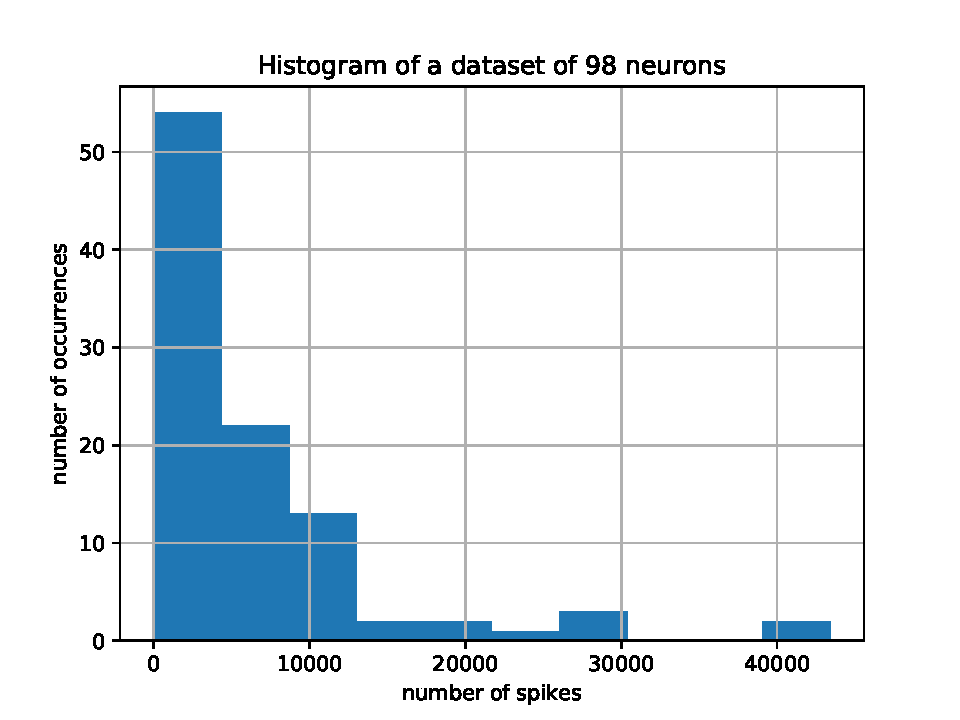
\includegraphics[width=0.8\textwidth]{histogram_number_spikes_dataset.pdf}
	\caption{Histogram of the number of spikes in a network of 98 neurons}
	\label{fig:histogram_spikes}
\end{figure}

\section{Input stimulus to the system}\label{sec:input_stimulus}

Previous work \cite{alexandru2018estimating} simulated a network whose input was a DC voltage that stimulated each of the neurons one by one for a defined period of time (4 seconds). This proved to be very useful because it facilitated the analysis of each of the neurons regardless of their level of connectivity and because it provided a systematic way of generating cascades (more on this in section \ref{sec:simulating_cascade_generation}).
However, the neural system cultures from the dataset are not stimulated. Instead, they are left alone to interact between each other. The neurons then communicate independently of the outside environment and spike at a lower frequency as a result. \\

The input stimulus cannot be left unchanged because the behaviour of the network would be radically different to that of the real one. It cannot be null either because then no interactions between the neurons would occur. Some type of random input noise must be present in order to have spikes. Moreover, the new model should have biological significance since a real network is being replicated. An option is investigated that could potentially meet these requirements.\\

\subsection{System with random spikes}\label{sec:sys_rand_spikes}

The proposed model intends to mimic biological behaviour by assuming that neurons spike when they want to transmit some information that they have conveyed by themselves. In order to do so, a random neuron is selected from the network and stimulated with random noise for some length of time.
The benefit of this model arises from its ability to insure that every neuron has roughly the same probability of originating a spike train, from its random behaviour in the system and from its major biological resemblance than the model used in \cite{alexandru2018estimating}.\\

The noise that is input to the selected neuron is taken from the absolute value of a normal distribution of zero mean and standard deviation equal to \(\alpha\). Since, a model of only excitatory neurons is being implemented, negative values from the distribution are not valid. \\

The amount of time the selected neuron is stimulated for is also random. It is taken from a uniform distribution in the range 0 to 200 ms. There is no evidence to support the selection of this number since to this day, the behaviour of the neuron is not very well understood. However, it must be sufficiently large for the neuron to spike but to not too big so as to allow other neurons to be stimulated too. \\



\section{Number of spikes}\label{sec:number_of_spikes}

It can be seen in table \ref{tab:spike_characteristics} that one of the most obvious differences between the real dataset and the previous simulations is the total number of spikes. The number is significantly smaller than before even though the observation time is larger. This is because the stimulation model forced the neurons to spike very frequently. In \cite{alexandru2018estimating} the total observation time was equal to the defined length of stimulation multiplied by the number of neurons. Since the stimulation period was found to be optimal for 4 seconds, then for a network of 98 neurons, this would result in a total of 392 seconds of recordings. \\ 

\begin{table}[]
\centering
\begin{tabular}{|c|c|c|c|c|c|}
\hline
Type of network  & Neurons & Duration & Number of spikes & Mean    & Freq spikes/neuron \\ \hline
Real             & 98                & 3600 s           & 636878           & 6498.2  & 1.2 Hz               \\ \hline
Sim. DC stimulus & 98                & 392 s            & 4038313          & 41207.3 & 105.12 Hz            \\ \hline
\end{tabular}
\caption{Spike characteristics of different types of neural networks}
\label{tab:spike_characteristics}
\end{table}

On the other hand, the real dataset consists of recordings of one hour. Therefore, the model of the simulation must be such that the number of spikes is roughly the same for a 1 hour simulation length. This can be achieved by varying the parameter \(\alpha\) from the input stimulus of the model. This variable controls the standard deviation of the absolute normal distribution defined in section \ref{sec:sys_rand_spikes}. The larger it is, the more voltage will be induced into the neuron and the higher its probability of spiking.
Every simulation will have a considerably different number of spikes given the parameter \(\alpha\). However, its effect on the number of spikes is investigated for a 1 hour simulated network of 98 neurons. This will give a rough estimate of what the parameter value should be. Figure \ref{fig:I_var_plot} shows that the most appropriate value of \(\alpha\) is 4. 

\begin{figure}[H]
	\centering
	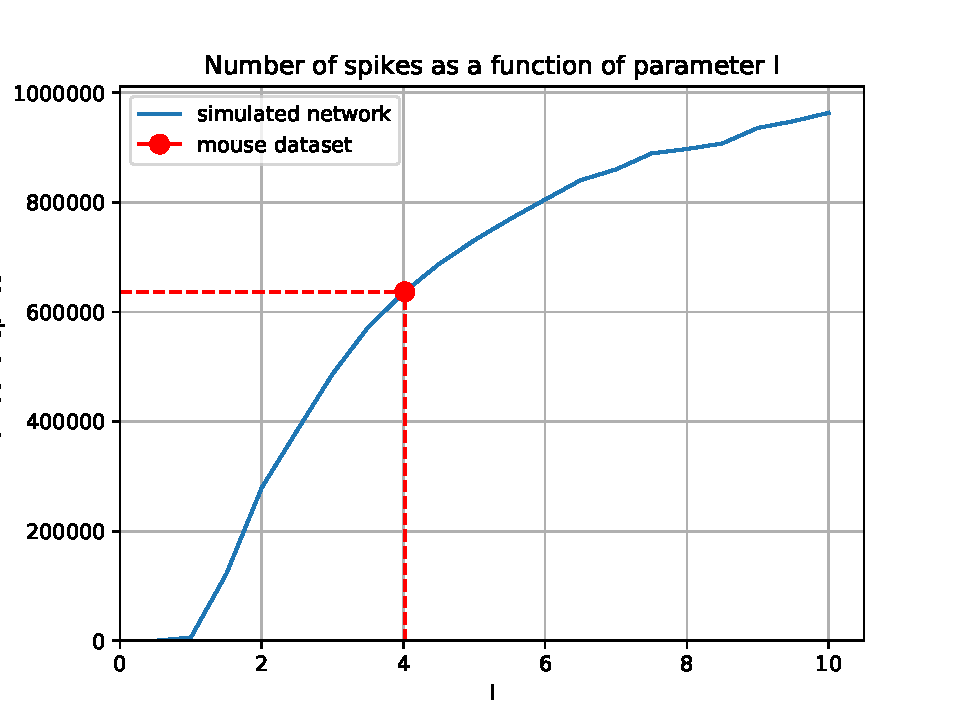
\includegraphics[width=0.8\textwidth]{I_var_plot.pdf}
	\caption{Number of spikes as a function of the parameter I for a 1 hour simulated network of 98 neurons and a random spike stimulus}
	\label{fig:I_var_plot}
\end{figure}


% Number of spikes
% 	I_var
% 	Frequency of spikes
% Shape of the histogram
% 	Changing the randomisation of the adjacency weights
% Types of neurons
% 	Excitatory and inhibitory
% 	What type of excitatory



\section{Cascade generation}\label{sec:simulating_cascade_generation}

Once the network model is defined what remains to clarify is how the cascades will be built. The method used in \cite{alexandru2018estimating} was simple and consistent. Since a DC stimulus was given to one neuron at a time, this neuron was selected to be the beginning of the cascade. This cascade would last for \(T\) length of time and only the first firing of each neuron would be taken into account. This insures that the third assumption from \cite{rodriguez2011uncovering} is not broken, i.e observable artefacts in are binary. Moreover, with this cascade generation method, cascade independence was guaranteed because it provided a clear entry point into the diffusion process. Since the system no longer has a DC input, the cascade generation method must be changed. When selecting an appropriate method of cascade generation, certain factors need to be taken into account.
\begin{enumerate}
\item The higher the number of cascades that are generated, the more information will be conveyed and, in general, the better NetRate will be able to infer the connectivity of the network. 
\item The more separated the cascades are from each other in the time domain, the more independent they will be. In \cite{rodriguez2011uncovering}, independence is defined as uniqueness of spikes for all the cascades in the diffusion process. However, for this project, an additional definition will be used i.e the level of isolation between the different diffusion processes in the time series. Now, a set of independent cascades not only contains unique spikes but, each of the cascades in the set has no influence over each other.
\item A high sparsity insures that enough cascade information is obtained from all the neurons in the network. Otherwise, only neurons who spike often will be the ones generating cascades.
\end{enumerate}

\subsection{Method of maximum cascades}

One way of building cascades is the proposed method of maximum cascades. This is a very simple approach that uses the first spiking neuron as the beginning of the cascade. This cascade lasts for the defined horizon and includes all the firing activity within this time period. This process is repeated after the last spike of the generated cascade and until the whole time series has been evaluated. It is worth remembering that, in the case of one neuron firing twice within the same time period, only the first one is taken into account and recorded in the cascade. As an example, let there be a network of 5 neurons that spike during a recording of 12 seconds and let the firing times and neuron indices be:

\begin{align}
	\centering
	firings = &\{1.5, 2.6, 4.7, 8.1, 8.4, 9.4, 11.2\}\\
	indices = &\{4,  3,  5,  3,  2,  2, 4\}
\end{align}

Then, using the method of maximum cascades, the resulting two cascades would be the ones seen below:

\begin{align}
	\centering
	\textbf{t}^{1} = &\{\infty, \infty, 1.1, 0, 3.2 \}\\
	\textbf{t}^{2} = &\{\infty, 0.3, 0, 2.1, \infty \}
\end{align}

The first cascade starts at time \(t=1.5s\) and ends at \(t=6.5s\). During this time, neurons 3, 4 and 5 spike. Then, the second cascade, starts at time \(t=8.4s\) and finishes at \(t=12s\). Here, neurons 2, 3 and 4 spike. However, although neuron 2 spikes twice, only the first firing is taken into account. It is also worth remembering that, cascades are based on time differences rather than absolute times. \\

The advantage of this method stems from the large number of cascades that are generated. Every spike is used for generating cascades and, thus, the number of cascades is maximized. However, this is done irrespective of their quality. The quality of a cascade is defined as the fidelity of the probabilistic description of the network. In other words, how well it represents the true nature of the system. As an example, let the firings and indices of a simulation of 20 seconds with a horizon of 10 seconds be the ones in \ref{eq:quality_cascades} and let the network connections be the ones in table \ref{tab:quality_cascades}.

\begin{align}
	\centering
	firings = &\{1, 9, 11, 12, 19\}\\
	indices = &\{1, 2,  3,  4, 2\}
	\label{eq:quality_cascades}
\end{align}

\begin{table}[H]
\centering
\begin{tabular}{|c|c|}
\hline
Source & Target \\ \hline
1      & 2      \\ \hline
1      & 4      \\ \hline
2      & 3      \\ \hline
2      & 4      \\ \hline
3      & 2      \\ \hline
\end{tabular}
\caption{Network connections example}
\label{tab:quality_cascades}
\end{table}

The resulting cascades would then be:

\begin{align}
	\centering
	\textbf{t}^{1} = &\{0, 8, \infty, \infty \}\\
	\textbf{t}^{2} = &\{\infty, 8, 0, 1 \}
\end{align}

Although the above cascades are well constructed, the second cascade is of poor quality. This is because, under a deterministic model where there is no noise, the cascade would lead to believe that there is a connection between nodes 3 and 4 when, in fact, the spiking of node 4 was caused by either node 1 or 2. Since NetRate is made for inferring networks under stochastic conditions, this scenario could happen under an otherwise perfect system. However, the cascade method of maximum cascades is fundamentally flawed because cascades are not independent. The diffusion process from the first cascade has not reached a steady state and it has affected the second cascade. A new cascade method is proposed where the independence of cascades is increased. 



\subsection{Method of optimal independence}

Under the new definition, independence of cascades cannot be guaranteed. Any spiking activity could cause another neuron to become unstable in the future or could, at least, contribute to this happening by increasing its membrane potential. However, it can be improved significantly by allowing the network to reach a steady state before starting the cascade.\\

The method of optimal independence poses a stability constraint on cascade generation. This is achieved by requiring the first spike of each cascade to be a specific amount of time far away from its immediate previous spike. For simplicity, in this project, this time variable will be equal to the time horizon used as the duration of the cascade.\\

This method increases the quality of the cascades in comparison to the one of maximum cascades. However, since it is more difficult to generate cascades that meet the requirements, there will also be fewer cascades. This is not always a problem, since, many times the number of cascades generated by the first method exceeds the computation capabilities of the computer at hand. By modifying the stability period parameter, the number of desired cascades can be chosen and only the ones with the highest independence will be used.

\section{Concluding remarks}

At the beginning of this chapter the need for a simulated network that approximated the biological one was explained. Such a model can provide an approximation of performance of the algorithm. It is based on the assumption that the simulation is a faithful representation of the real nature of the network. Moreover, the differences between previous simulated networks and this new real network make it vital to verify that the algorithm would still work under these new conditions. \\

A new model was defined that tries to mimic the behaviour of the real mouse recordings. For this reason, instead of simulating a network whose input consisted of a DC stimulus, a random input was established that consisted of the absolute value from a normal distribution of mean zero and standard deviation \(\alpha\). This stimulus would be given for a random amount time to a random neuron in the system. \\

Finally, two new methods of cascade generation were defined. This was necessary because the change of input stimulus made the previous approach obsolete. The proposed method of \textit{maximum cascades} constructs cascades based on the firing times of the neurons and allows a large number of cascades to be generated. Finally, the method of \textit{optimal independence} poses a constraint on the stability of the system thereby increasing the quality of the cascades.







